%\setbeamertemplate{navigation symbols}{} %to remove beamer navigation
%\setbeamertemplate{footline}[frame number] %adds frame number BELOW navigation buttons
%\usetheme{Singapore}
%\usetheme{Pittsburgh}
%\usetheme{boxes}
%\usepackage[utf8]{inputenc}
%\usepackage{amsmath}
%\usepackage{amsfonts}
%\usepackage{amssymb}
%\usepackage{graphicx}
\usepackage{tikz}     %Used for drawing tikzpictures
\usepackage{multirow} %Used for tables with merged cells
\usepackage{collcell} %pdflatex.exe hangs without this one
\usepackage{ulem}     %Used for \sout to strikethrough font
%\usepackage{xcolor}   %Can be used for \colorbox{green}{highlighted text}
%\setbeamercovered{transparent}
%\setbeamertemplate{navigation symbols}{}
%\logo{}
%\date{}
%\subject{}
\title{RS: Elementary \newline \newline (Network Administrator Series)}

\begin{document}

%\includeonlyframes{current}
\author{Alexandr Alakin}
\institute[BASU]{BAS University}

% Use \wiki{OSI model}{OSI_model} to create a link named "OSI model" to Wikipedia page (OSI_model)
% At the end of this link a Wiki logo will be added as well
\newcommand{\wiki}[2]{\href{https://en.wikipedia.org/wiki/#2}{#1
\includegraphics[scale=0.21]{../common/images/wiki_letter.png}}}

% Use \rfc{791} to create a link named "RFC971" to https://tools.ietf.org/html/rfc791
\newcommand{\rfc}[1]{\href{https://tools.ietf.org/html/rfc#1}{RFC#1}}

\def\Gobble#1\EndGobble{}

\begin{frame}
	\titlepage
\end{frame}

\begin{frame}{Table of contents}
	\pdfbookmark[2]{Table of contents}{toc}
	\begin{spacing}{0.1}
		\tableofcontents[hideallsubsections]
	\end{spacing}
\end{frame}

\begin{frame}
	\frametitle{Contacts}
	\texttt{
		\begin{tabular}{l|l}
			Email 	& a@bas.kz	\\ \hline
			Skype 	& a.bas.kz	\\
		\end{tabular}
	}
\end{frame}

\section[intro]{Introduction}

\begin{frame}{Introduction}
	\begin{itemize}[<+->]
		\item Prerequisites:
		\begin{itemize}
			\item No strict requirements
		\end{itemize}
		\item Course goals:
		\begin{itemize}
			\item Network fundamentals
			\item Switching
			\item Routing
			\item Security
			\item IPv6
		\end{itemize}
		\item Timing and environment:
		\begin{itemize}
			\item Start, end, coffee breaks, lunch
			\item Phones, Wi-Fi
		\end{itemize}
		\item Introduce Yourself:
		\begin{itemize}
			\item Experience
			\item Goals
		\end{itemize}
	\end{itemize}
\end{frame}

\AtBeginSection[]{
	\begin{frame}<beamer>
		\frametitle{Plan}
		\tableofcontents[
			currentsection,
			currentsubsection,
			subsectionstyle=show/show/hide
		]
	\end{frame}
}
\section[meet]{Meet the Network}

\begin{frame}{Network Components}
	\begin{itemize}[<2->]
		\item Router
		\item Switch
		\item Access Point (AP)
		\item Firewall
		\item Network Interface Card (NIC)
	\end{itemize}
	\begin{itemize}[<3->]
		\item Personal Computer (PC)
		\item Laptop
		\item Server
	\end{itemize}
	\begin{itemize}[<4->]
		\item Copper
		\item Fiber Optic
		\item Radio Frequency
	\end{itemize}
\end{frame}
\begin{frame}{Network Characteristics}
	\begin{itemize}[<+->]
		\item Size vs Scalability
		\item Topology (physical vs logical)
		\item Security:
		\begin{itemize}
			\item Data traffic security
			\item Network device security
		\end{itemize}
		\item Reliability of a single device
		\item Availability of a service
	\end{itemize}
\end{frame}

\begin{frame}{Diagram of the First Internetworked Connection}
	\begin{figure}
		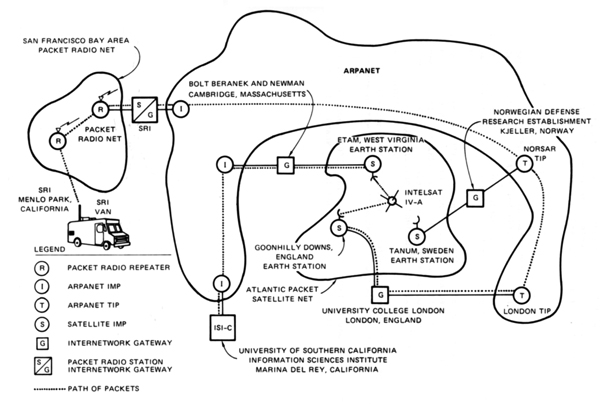
\includegraphics[width=300pt]{../common/images/SRI_First_Internetworked_Connection_diagram.jpg}\\
		{\scriptsize https://en.wikipedia.org/wiki/File:SRI\_First\_Internetworked\_Connection\_diagram.jpg}
	\end{figure}
\end{frame}

\begin{frame}{Network Protocols}
	\begin{itemize}[<+->]
		\item Set of rules for transmission of information over media
		\item Examples:
		\begin{itemize}
			\item Ethernet (\wiki{IEEE 802.3}{IEEE_802.3})
			\item Internet Protocol (IP, \rfc{791})
			\item Address Resolution Protocol (ARP, \rfc{826})
			\item Dynamic Host Configuration Protocol (DHCP, \rfc{2131})
			\item Domain Name System (DNS, \rfc{1034}, \rfc{1035})
			\item Open Shortest Path First (OSPF, \rfc{2328})
			\item Border Gateway Protocol (BGP, \rfc{4271})
			\item Internet Protocol version 6 (IPv6, \rfc{2460})
		\end{itemize}
	\end{itemize}
\end{frame}
\begin{frame}{Communication Models}
	\begin{itemize}[<+->]
		\item Open Systems Interconnection model (\wiki{OSI model}{OSI_model})
		\item Internet protocol suite (\wiki{TCP/IP stack}{IP_stack}, \rfc{1122})
	\end{itemize}
	\onslide<3-4>
	\begin{center}
	\newcolumntype{G}{|l}
	\only<beamer>{ \only<3>{\newcolumntype{G}{@{}>{\Gobble}l<{\EndGobble}@{}}} }

	\begin{tabular}{G|l|l|l|}
	\hline
		\textbf{Mnemonic}&  \textbf{\#} & \textbf{OSI} & \textbf{TCP/IP}              \\ \hline
		All              &  7           & Application  & \multirow{3}{*}{Application} \\ \cline{1-3}
		People           &  6           & Presentation &                              \\ \cline{1-3}
		Seem             &  5           & Session      &                              \\ \hline
		To               &  4           & Transport    & Transport                    \\ \hline
		Need             &  3           & Network      & Internet                     \\ \hline
		Data             &  2           & Data Link    & \multirow{2}{*}{Link Access} \\ \cline{1-3}
		Processing       &  1           & Physical     &                              \\ \hline
	\end{tabular}
	\end{center}
\end{frame}
\begin{frame}{Data Flow}
	\begin{figure}
		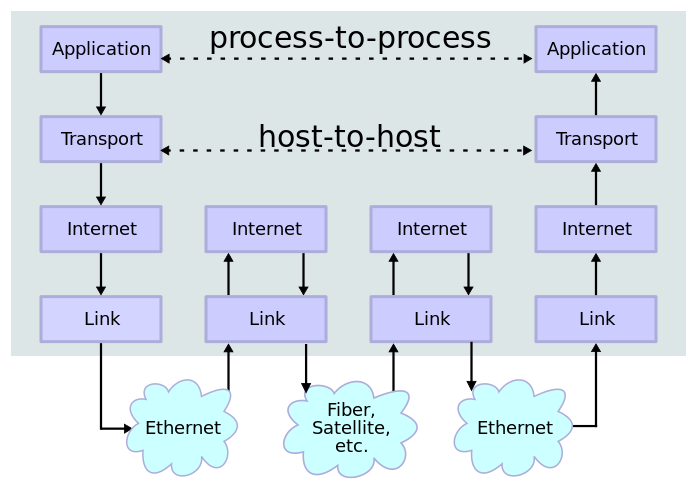
\includegraphics[width=300pt]{../common/images/IP_stack_connections_flow.png}\\
		{\scriptsize https://en.wikipedia.org/wiki/File:IP\_stack\_connections.svg}
	\end{figure}
\end{frame}
\begin{frame}{Wireshark Capture}
	\begin{figure}
		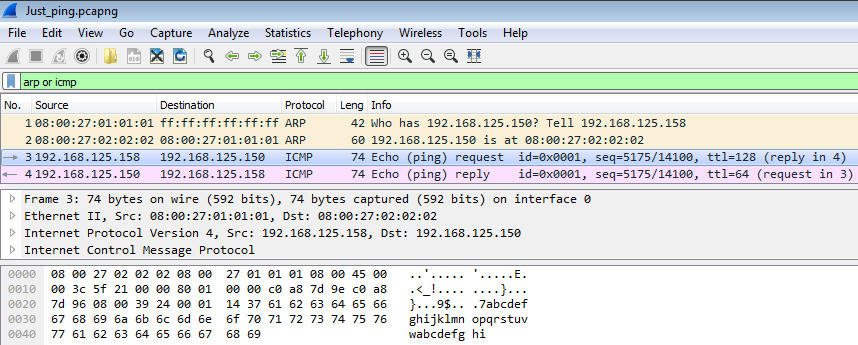
\includegraphics[width=300pt]{../common/images/Wireshark__ARP_or_ICMP.png} \newline \newline
		Get Wireshark at \texttt{\href{https://wireshark.org/}{https://wireshark.org/}}
	\end{figure}
\end{frame}
\begin{frame}<handout:0>{Wireshark Capture (Cont.)}
	\begin{figure}
		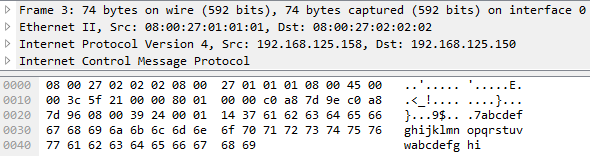
\includegraphics[width=300pt]{../common/images/Wireshark__ARP_or_ICMP_zoom.png}
	\end{figure}
\end{frame}
\begin{frame}<handout:0>{Wireshark Capture (Cont.)}
	\begin{figure}
		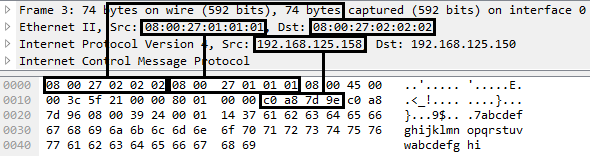
\includegraphics[width=300pt]{../common/images/Wireshark__ARP_or_ICMP_zoom_with_lines.png}
	\end{figure}
\end{frame}

\section[ipv4]{Layer 3 (Internet Protocol)}

\subsection{IP, IP Address and Subnet Mask}
\begin{frame}{IP, IP Address and Subnet Mask}
	\wiki{Internet Protocol}{Internet_Protocol} \wiki{Address}{IPv4\#Addressing}\pause
	\begin{itemize}[<+->]
		\item \rfc{791}
		\item 32-bit length (4 294 967 296 addresses)
		\item Divided into 4 octets (bytes)
		\item Each octet is converted from binary to decimal
		\item \texttt{00001010 00000001 00000001 01100100}
		\item 10.1.1.100
		\item Identification of any host on a network
	\end{itemize}
	\onslide<9->
	Mask\pause
	\begin{itemize}[<+->]
		\item 32-bit length
		%\item In binary: '1' is not allowed after '0'
		\item \texttt{11111111 11111111 11111111 00000000}
		\item 255.255.255.0
	\end{itemize}
\end{frame}

\subsection{Binary-Decimal-Binary conversion}
\begin{frame}{Binary-Decimal-Binary conversion}
	\textit{There are 10 types of people in the world. Those who understand binary and those who don't.}
	\pause
	\texttt{
		\begin{center}
			\begin{tabular}[t]{r}
				Decimal \\ \pause
				{[0-9]}	\\ \pause
				0	\\ \pause
				1	\\ \pause
				2	\\ \pause
				...	\\ \pause
				9	\\ \pause
				10	\\ \pause
				... \\ \pause
				99	\\ \pause
				100\\ \pause
			\end{tabular}
			\hspace{1.5cm}
			\begin{tabular}[t]{r r}
				Decimal		&	Binary	\\
				{[0-9]}		&	[0-1]	\\ \hline \pause
				0	\pause	&	0		\\ \pause
				1	\pause	&	1		\\ \pause
				2	\pause	&	10		\\ \pause
				3	\pause	&	11		\\ \pause
				4	\pause	&	100		\\ \pause
				5	\pause	&	101		\\ \pause
				6	\pause	&	110		\\ \pause
				7	\pause	&	111
			\end{tabular}
		\end{center}
	}
\end{frame}

\begin{frame}{Binary to Decimal conversion}
	\texttt{
		\begin{center}
			\begin{tabular}{*{9}c}
				2\textsuperscript{7} & 2\textsuperscript{6} & 2\textsuperscript{5} &
				2\textsuperscript{4} & 2\textsuperscript{3} & 2\textsuperscript{2} &
				2\textsuperscript{1} & 2\textsuperscript{0} \\ \pause
				128 & 64 & 32 & 16 & 8 & 4 & 2 & 1 \\ \pause
				  0 &  1 &  0 &  0 & 0 & 1 & 0 & 1 \\ \pause
				    & 64 &    &    &   & 4 &   & 1 \pause & 69 \\
			\end{tabular}
		\end{center}
	}
\end{frame}

\begin{frame}{Decimal to Binary conversion}
	\only<beamer>{\only<1>{\textit{Change analogy}}}
	\pause
	\texttt{
		\begin{center}
			\begin{tabular}{*{9}c}
				          & 128 & 64 & 32        & 16 &  8        & 4        & 2        & 1 \\
				46 \pause &     &    & 46 \pause &    & 14 \pause & 6 \pause & 2 \pause &   \\
				          &   0 &  0 &  1        &  0 &  1        & 1        & 1        & 0 \\
			\end{tabular}
		\end{center}
	}
\end{frame}

\subsection{Meaning of the Mask}
\begin{frame}{Meaning of the Mask}
	\texttt{
		\onslide<3->{\\10.1.1.100 255.255.255.0}
		\onslide<4->{\\10.1.1.100/24\vspace{0.2cm}}
		\only<9->{\\10.1.1.0\\10.1.1.1\\10.1.1.254\\10.1.1.255\vspace{0.2cm}}
		\only<1,3->{\\00001010 00000001 00000001 01100100\hspace{0.5cm}IP Address}
		\only<2|handout:0>{\\00001010 00000001 00000001\colorbox{green}{01100100}\hspace{0.5cm}IP Address}
		\onslide<2->{\\11111111 11111111 11111111 00000000\hspace{0.5cm}Mask
		\onslide<5->{\noindent\rule[0.5ex]{\linewidth}{0.7pt}}
		\onslide<5->{\\00001010 00000001 00000001 00000000\hspace{0.5cm}Network Ad.}
		\onslide<7->{\\00001010 00000001 00000001 00000001\hspace{0.5cm}First Ad.}
		\onslide<8->{\\00001010 00000001 00000001 11111110\hspace{0.5cm}Last Address}
		\onslide<6->{\\00001010 00000001 00000001 11111111\hspace{0.5cm}Broadcast}
		}
	}
\end{frame}

\subsection{Cisco Commands}
\begin{frame}{Commands: Hostname, IP Address, Save Config}
	\texttt{
		\only<2-3|handout:0>{\pause\\\textit{Press RETURN to get started}
		\vspace{0.5cm}}
		\pause\\Router>\onslide<4->{\underline{en}able} \hfill \only<3,5->{User EXEC mode}\only<4|handout:0>{Go to Privileged EXEC}
		\pause\pause\pause\\Router\#\onslide<5->{\underline{conf}igure \underline{t}erminal} \hfill Privileged EXEC mode
		\pause\\Router(config)\#hostname R\hfill Configuration mode
		\pause\\R(config)\#\pause interface GigabitEthernet0/1
		\pause\\R(config-if)\#ip address 10.1.1.1 255.255.255.0
		\pause\\R(config-if)\#no shutdown
		\pause\\R(config-if)\#exit \only<beamer>{\hfill or \underline{end} to go to \#}
		\pause\\R(config)\#exit
		\pause\\R\#show startup-config
		\pause\\R\#show running-config \pause {[ interface \{ gi0/1 \} ]}
		\pause\\R\#show ip interface [ gi0/1 | brief [ gi0/1 ] ]
		\pause\\R\#copy running-config startup-config
		\pause\\Destination filename [startup-config]?%\hfill <ENTER>
		\pause\\Building configuration...
		\\{[OK]}
		%\pause\\
	}
\end{frame}

\subsection{Types and Classes of IP Addresses}
\begin{frame}{Types and Classes of IP Addresses}
	\begin{itemize}[<+->]
		\item Localhost: Local communications only (127.0.0.0/8)
		\item Unicast: One-to-one communication (e.g. 10.1.1.1)
		\item Multicast: One-to-many communication (e.g. 224.0.0.9)
		\item Local Broadcast: One to all local hosts (255.255.255.255)
		\item Directed Broadcast: One to all hosts in remote network (e.g. 172.16.255.255)
	\end{itemize}
	%\vspace{0.5cm}
	\onslide<6->{
		\begin{center}
			\begin{tabular}{*{9}l}
				Class & First bits &        First octet & Default mask    \\ \pause
				A     & 0          & \pause 1-126       & 255.0.0.0       \\ \pause
				B     & 10         & \pause 128-191     & 255.255.0.0     \\ \pause
				C     & 110        & \pause 192-223     & 255.255.255.0   \\ \pause
				D     & 1110       & \pause 224-239     & Multicast range \\ \pause
				E     & 1111       & \pause 240-255     & Reserved
			\end{tabular}
		\end{center}
	}
\end{frame}

\subsection{IP Routing}
\begin{frame}{IP Routing}
	\begin{itemize}[<+->]
		\item \wiki{Packet switching}{Packet_switching}
		\item \texttt{show ip route} (EXEC command) shows routing table
		\item C (Connected) routes are "interface" routes
		\item Routers can only reach known networks
		\item If destination address of an incoming packet is not in the routing table, then the packet is dropped
		\item Routers should "learn" all routes they need using:
		\begin{itemize}
			\item Static routing (manual configuration):
			\begin{itemize}
				\item \texttt{)\#ip route 192.168.1.0 255.255.255.0 10.1.1.2}
			\end{itemize}
			\item Dynamic routing (automatically):
			\begin{itemize}
				\item RIP
				\item EIGRP
				\item OSPF
				\item BGP
			\end{itemize}
		\end{itemize}
	\end{itemize}
\end{frame}

\subsection{Default Gateway}
\begin{frame}{Default Gateway}
	\begin{itemize}[<+->]
		\item Communication to hosts in the same network (identical network bits) is direct
		\item Communication to hosts outside local network is via default gateway (should be in the same network)
		\item 10.1.1.100/24 $\rightarrow$ 10.1.1.200 [Direct or via DG]?
		\item 10.1.1.100/24 $\rightarrow$ 10.1.2.200 [Direct or via DG]?
		\item 10.1.1.100/24 $\rightarrow$ 10.2.1.200 [Direct or via DG]?
		\item 10.1.1.100/24 $\rightarrow$ 20.1.1.200 [Direct or via DG]?
		\item \texttt{)\#ip route 192.168.1.0 255.255.255.0 10.1.1.1}
		\item \texttt{)\#ip route 192.168.0.0 255.255.0.0~~~10.1.1.1}
		\item \texttt{)\#ip route 192.0.0.0~~~255.0.0.0~~~~~10.1.1.1}
		\item \texttt{)\#ip route 0.0.0.0~~~~~0.0.0.0~~~~~~~10.1.1.1}
		\item \texttt{)\#ip default-gateway 10.1.1.1}
	\end{itemize}
\end{frame}

\section[ethr]{Layer 2 (Ethernet)}

\subsection{Cabling and Connectors}
\begin{frame}{Cabling and Connectors}
	Cables:\pause
	\begin{itemize}[<+->]
		\item \wiki{Coaxial cable}{Coaxial_cable}
		\item \wiki{Twisted pair}{Twisted_pair}
		\item \wiki{Optical fiber cable}{Optical_fiber_cable}
	\end{itemize}
	\onslide<5->{\vspace{0.5cm}Connectors:}\pause
	\begin{itemize}[<+->]
		\item \wiki{Twisted pair connectors}{Modular_connector\#8P8C}
		\begin{itemize}
			\item \wiki{T568A/T568B}{TIA/EIA-568\#Wiring}
			\item Straight-through cable
			\begin{itemize}
				\item Hubs/Switches to other devices
			\end{itemize}
			\item Crossover cable
			\begin{itemize}
				\item Hubs/Switches to Hubs/Switches
				\item Other devices to other devices
			\end{itemize}
		\end{itemize}
		\item \wiki{Optical fiber connector}{Optical_fiber_connector}
	\end{itemize}
\end{frame}

\subsection{Collisions and duplex}
\begin{frame}{Collisions and duplex}
	\wiki{Carrier-sense multiple access with collision detection (CSMA/CD, half-duplex)}{Carrier-sense_multiple_access_with_collision_detection}\pause
	\begin{itemize}[<+->]
		\item Is medium idle?
		\item Transmit a frame and monitor for collision
		\item If collision occurs:
		\begin{itemize}
			\item Send jam signal (make sure collision is detected)
			\item Wait random time (based on number of attempts)
			\item Try sending the frame again
		\end{itemize}
	\end{itemize}
	\onslide<8->{\wiki{Half-duplex}{Half-duplex}}\pause
	\begin{itemize}[<+->]
		\item CSMA/CD
		\item Hub
	\end{itemize}
	\onslide<11->{\wiki{Full-duplex}{Full-duplex}}\pause
	\begin{itemize}[<+->]
		\item \sout{CSMA/CD}
		\item Switch
	\end{itemize}
\end{frame}

\subsection{Ethernet frame structure}
\begin{frame}{Ethernet frame structure}
	\wiki{Ethernet frame}{Ethernet_frame} structure\pause
	\begin{itemize}[<+->]
		\item Preamble (7 bytes)
		\item Start of frame delimiter (1 byte)
		\item MAC destination (6 bytes)
		\item MAC source (6 bytes)
		\item Ethertype (2 bytes)
		\item Payload (46-1500 bytes)
		\item Frame check sequence (4 bytes)
		\item Interpacket gap (12 bytes)
	\end{itemize}
	\only<10-|handout:0>{Wireshark lab\pause
		\begin{itemize}[<+->]
			\item Which fields are not shown in Wireshark and why?
		\end{itemize}
	}
\end{frame}

\subsection{Structure and types of MAC addresses}
\begin{frame}{Structure and types of MAC addresses}
	\wiki{MAC address}{MAC_address} structure\pause
	\begin{itemize}[<+->]
		\item Total length is 6 bytes (48 bits, 12 hex characters)
		\item First half is Organisationally Unique Identifier (OUI)
		\begin{itemize}
			\item 7th bit (U/L or LG bit) shows if address is universally/globally (0) or locally administered (1)
			\item 8th bit (U/M or IG bit) determines unicast/individual (0) or multicast/group (1) frame
		\end{itemize}
		\item Second half is NIC specific
	\end{itemize}
	\onslide<7->{MAC address types}\pause
	\begin{itemize}[<+->]
		\item Unicast (received by single host)
		\item Multicast (received by multiple hosts)
		\item Broadcast (received by all hosts)
	\end{itemize}
	\only<11-|handout:0>{Wireshark lab\pause
		\begin{itemize}[<+->]
			\item Find OUI, LG and IG fields
		\end{itemize}
	}
\end{frame}

\subsection{Ethernet Switches}
\begin{frame}{Ethernet Switches}
	\begin{itemize}[<+->]
		\item Process frames based on MAC Address Table state:
		\begin{itemize}
			\item Flood (send frame from one port to all other ports) unknown unicast, multicast and broadcast
			\item Forward (send frame from one port to another) known unicast
			\item Filter (do not send anywhere) frames which do not need to be forwarded
		\end{itemize}
		\item Learn MAC Addresses (fill MAC Addres Table)
	\end{itemize}
	\onslide<6->
	\texttt{
		\\      \#show interface status
		\\\pause\#show mac address-table interface \textit{type number}
		\\\pause\#show mac address-table address \textit{mac-addr}
	}
	\\\vspace{0.3cm}
	\hspace{2cm}
	\begin{tabular}{ll}
		  \pause \texttt{Interface}	&\texttt{MAC Address}
		\\\pause \texttt{Gi0/5}		&\texttt{0123.4567.89ab}
		\\\pause \texttt{Gi0/%
		 \only<11>          {6}%
		 \only<12|handout:0>{5}}	&\texttt{0123.4567.89ac}
	\end{tabular}\\
\end{frame}

\subsection{Port Security}
\begin{frame}{Port Security}
	Restricts input to an interface by limiting and identifying MAC addresses
	\vspace{0.3cm}
	\texttt{
		\\\pause )\#interface FastEthernet0/2
		\\\pause -if)\#\underline{sw}itchport mode access
		\\\pause -if)\#sw \underline{po}rt-security maximum \textit{maximum}
		\\\pause -if)\#sw po mac-address \textit{mac-addr}
		\\\pause -if)\#sw po mac-address sticky \pause\textit{[mac-addr]}
		\hangindent=2em{
		\\\pause -if)\#sw po violation \{ protect | restrict | shutdown \}}
		\\\pause -if)\#switchport port-security
	}
	\\\vspace{0.1cm}\hspace{1.5cm}
	\begin{tabular}{l*{3}c}
		        \pause Violation	&Drop	&Log	&Error-disable
		\\\hline\pause Protect		&Yes
		\\      \pause Restrict		&Yes	&Yes
		\\      \pause Shutdown*		&Yes	&Yes	&Yes
	\end{tabular}\\
\end{frame}

\begin{frame}{Port Security (Cont.)}
	\texttt{
		\\\#show interface [\textit{ type number }] status
		\\\pause Port~~~~~~Name~~~~~Status
		\\       Fa0/1~~~~~~~~~~~~~~connected
		\\       Fa0/2~~~~~~~~~~~~~~notconnect
		\\       Fa0/3~~~~~~~~~~~~~~disabled
		\\       Fa0/4~~~~~~~~~~~~~~err-disabled\vspace{0.3cm}
		\\\pause \#show interface status err-disabled
		\\\pause Port~~~~~~Name~~~~~Status~~~~~~~Reason
		\\       Fa0/4~~~~~~~~~~~~~~err-disabled~psecure-violation
	}
	\\\vspace{0.3cm}\pause
	To bring interface back either \texttt{shutdown/no shutdown} interface or use automatic error-disable recovery feature:
	\pause\vspace{0.3cm}
	\texttt{
		\\)\#errdisable recovery cause psecure-violation
		\\)\#errdisable recovery interval \textit{interval}
	}\\
\end{frame}

\section[locl]{Intranet Communications}

\subsection{Client-Server Applications and Protocols}

\begin{frame}{Client-Server Applications and Protocols}
	Examples:\pause
	\begin{itemize}[<+->]
		\item \wiki{World Wide Web}{World_Wide_Web} and \wiki{HTTP}{Hypertext_Transfer_Protocol}, \wiki{HTTPS}{HTTPS}
		\item \wiki{Electronic mail}{Email} and \wiki{SMTP}{SMTP}, \wiki{POP3}{Post_Office_Protocol}, \wiki{IMAP}{Internet_Message_Access_Protocol}
	\end{itemize}
	\onslide<4->
	Transport protocols (Layer 4):\pause
	\begin{itemize}[<+->]
		\item Client-Server port numbers
		\item \wiki{TCP}{Transmission_Control_Protocol}, \rfc{791}
		\begin{itemize}
			\item Three-way handshake
			\item Reliable transmission
			\begin{itemize}
				\item Sequence and acknowledge numbers
				\item Checksum and retransmission
			\end{itemize}
			\item Flow control
			\item Congestion control
		\end{itemize}
		\item \wiki{UDP}{User_Datagram_Protocol}, \rfc{768}
		\begin{itemize}
			\item Optional checksum
		\end{itemize}
	\end{itemize}
\end{frame}

\subsection{Dynamic Host Configuration Protocol}

\begin{frame}{Dynamic Host Configuration Protocol}
	\wiki{DHCP}{Dynamic_Host_Configuration_Protocol} (\rfc{2131}), allows automatic configuration of:\pause
	\begin{itemize}[<+->]
		\item IP address
		\item Mask
		\item Default gateway
		\item and more
	\end{itemize}
	\onslide<6->
	Important DHCP Messages\pause
	\begin{itemize}[<+->]
		\item Discover
		\item Offer
		\item Request
		\item Acknowledge
	\end{itemize}
	\onslide<11->
	DHCP uses UDP\pause
	\begin{itemize}[<+->]
		\item Port 68 for client
		\item Port 67 for server
	\end{itemize}
\end{frame}

\begin{frame}{Dynamic Host Configuration Protocol}
	Cisco IOS DHCP Client configuration
	\\\pause\texttt{-if)\#ip address dhcp}
	\\\vspace{0.5cm}\pause Cisco IOS DHCP Server configuration
	\texttt{
		\\\pause \hangindent=2em )\#ip dhcp excluded-address \textit{ip-address [last-ip-address]}
		\\\pause )\#ip dhcp pool \textit{name}
		\\\pause dhcp-)\#network \textit{network-number mask}
		\\\pause dhcp-)\#default-router \textit{address}
		\\\pause dhcp-)\#lease \textit{days [ hours [minutes] ]}
		\\\pause dhcp-)\#dns-server \textit{address}
		\\\pause dhcp-)\#domain-name \textit{domain}
	}\\\vspace{0.5cm}
	\pause Cisco IOS DHCP Relay configuration
	\\\pause\texttt{-if)\#ip helper-address \textit{address}}
\end{frame}
%}

\subsection{Virtual Local Area Networks}

\begin{frame}{VLANs}
	\texttt{
		\begin{columns}
			\begin{column}{0.5\textwidth}
				\begin{tabular}{l}
					\multicolumn{1}{c}{Unmanaged switch}\\
					\hline
					\multicolumn{1}{|c|}{1 2 3 4 5 6 7 8 9 10}\\
					\hline\pause\\
					\#show mac address-table\\
					\hline
					MAC1~~~Fa0/1\\
					MAC2~~~Fa0/2\\
					MAC5~~~Fa0/5\\
					MAC6~~~Fa0/6\\
					\hline
				\end{tabular}
			\end{column}
			\pause
			\begin{column}{0.5\textwidth}
				\begin{tabular}{lll}
					\multicolumn{3}{c}{Switch with VLAN support}\\
					\hline
					\multicolumn{1}{|l}{1 2 3}&\multicolumn{1}{|l}{4 5 6}&\multicolumn{1}{|l|}{7 8 9 10}\\
					\hline\pause\\
					\multicolumn{3}{l}{\#show mac address-table}\\
					\hline
					\multicolumn{3}{l}{VLAN123~~~MAC1~~~Fa0/1}\\
					\multicolumn{3}{l}{VLAN123~~~MAC2~~~Fa0/2}\\
					\hline
					\multicolumn{3}{l}{VLAN456~~~MAC5~~~Fa0/5}\\
					\multicolumn{3}{l}{VLAN456~~~MAC6~~~Fa0/6}\\
					\hline
				\end{tabular}
			\end{column}
		\end{columns}
		\pause\vspace{1cm}
		)\#vlan 2						\hfill	\textcolor<6->{black!50}{Create VLAN}
		\pause\\-vlan)\#name NEW-VLAN	\hfill	\textcolor<7->{black!50}{Rename VLAN}
		\pause\\-vlan)\#interface fa0/3
		\pause\\-if)\#switchport access vlan 3	\hfill	\textcolor<9->{black!50}{Assign VLAN}
		\pause\\\% Access VLAN does not exist. Creating vlan 3
	}
\end{frame}

\begin{frame}{Verifying VLAN and Port Status}
	\texttt{\#show vlan brief
		\pause\\VLAN~Name~~~~~~~Status~~~~Ports
		      \\----~----------~--------- ---------
		      \\1~~~~default~~~~active~~~~Fa0/1, Fa0/2, Fa0/4
		      \\2~~~~NEW-VLAN~~~active
		      \\3~~~~VLAN0003~~~active~~~~Fa0/3
		\vspace{0.5cm}
		\pause\\\#show interface status
		\pause\\Port~~~~~~Name~~~~~~Status~~~~~~~~~~~Vlan 
	          \\Fa0/1~~~~~~~~~~~~~~~connected~~~~~~~~1    
	          \\Fa0/2~~~~~~~~~~~~~~~connected~~~~~~~~1    
	          \\Fa0/3~~~~~~~~~~~~~~~connected~~~~~~~~3
	          \\Fa0/4~~~~~~~~~~~~~~~connected~~~~~~~~1
	}
\end{frame}

\begin{frame}{Access Ports and Trunks}
	\texttt{\framebox[1.1\width]{~frame1~}~~
			\framebox[1.1\width]{~frame2~}~~
			\framebox[1.1\width]{~frame3~} 
			\newline \pause
			\newline                     Fa0/1(1)~~~~Fa0/2(2)~~~~Fa0/3(3)~
			\newline\framebox[1.1\width]{~~~~~~~~~~~Switch~1~~~~~~~~~~~}\pause
			\newline\phantom{            ~~~~~~~~~~~~}Fa0/4(T)\newline\pause
			\newline\phantom{~~~~~~~}\framebox[1.1\width]{~frame1~\only<-7|handout:0>{|~VLAN~1~}}\only<8>{\hfill Native VLAN}
			\newline\phantom{~~~~~~~}\framebox[1.1\width]{~frame2~|~VLAN~2~}
			\newline\phantom{~~~~~~~}\framebox[1.1\width]{~frame3~|~VLAN~3~} 
			\newline\pause
			\newline\phantom{~~~~~~~~~~~~~}Fa0/4(T)
			\newline\framebox[1.1\width]{~~~~~~~~~~~Switch~2~~~~~~~~~~~}\pause
			\newline                     Fa0/1(1)~~~~Fa0/2(2)~~~~Fa0/3(3)~
			\newline\pause
			\framebox[1.1\width]{~frame1~}~~
			\framebox[1.1\width]{~frame2~}~~
			\framebox[1.1\width]{~frame3~} 
	}
\end{frame}

\begin{frame}{Trunk Encapsulations}
	\wiki{Ethernet Frame}{Ethernet_frame\#Structure}\\\vspace{0.1cm}
	\texttt{%
		\begin{tabular}{|c|c|c|c|c|c|}
			\hline 	6	&6	&2		&46-1500	&4\\
					DM	&SM	&Type	&Data		&FCS\\\hline
		\end{tabular}
	}
	\pause\\\vspace{0.5cm}\wiki{802.1Q Frame}{IEEE_802.1Q\#Frame_format}\\\vspace{0.1cm}
	\texttt{%
		\begin{tabular}{|c|c|c|c|c|c|}
			\hline 	6	&6	&4		&2		&46-1500	&4\\
					DM	&SM	&802.1Q	&Type	&Data		&FCS\\\hline
		\end{tabular}
	}
	\pause\\\vspace{0.5cm}\href{https://www.cisco.com/c/en/us/support/docs/lan-switching/8021q/17056-741-4.html}{ISL Frame}\\\vspace{0.1cm}
	\texttt{%
		\begin{tabular}{|c|c|c|c|c|c|c|c|}
			\hline 	26			&6	&6	&2		&46-1500	&4		&4\\
					ISL Header	&DM	&SM	&Type	&Data		&FCS	&ISL FCS\\\hline
		\end{tabular}
	}
\end{frame}

\begin{frame}{Configure and Verify Trunk Interfaces}
	\texttt{)\#int fa0/4
		\pause\\-if)\#switchport trunk encapsulation dot1q
		\pause\\-if)\#switchport trunk allowed vlan 2-3,8-10
		\pause\\-if)\#switchport trunk native vlan 99
		\pause\\-if)\#switchport mode trunk
		\pause\\-if)\#end
		\vspace{0.3cm}
		\pause\\\#show interface trunk
		\pause\\Port~~~~Mode~~~Encaps~~~Status~~~~~Native vlan
		      \\Fa0/4~~~on~~~~~802.1q~~~trunking~~~99
		      \vspace{0.3cm}
		      \\Port~~~Vlans allowed on trunk
		      \\Fa0/4~~2-3,8-10
		      \vspace{0.3cm}
		      \\Port~~~Vlans allowed and active
		      \\Fa0/4~~2-3
	}
\end{frame}

\subsection{IPv4 Routing}

\begin{frame}[label=current]{Routing}
	show ip route
\end{frame}


\end{document}
